 % Este arquivo é uma adaptação do modelo LaTeX disponibilizado pelo UTUG (http://www.inf.ufrgs.br/utug/)
% Autor: Prof. Dr. Adriel M. Ziesemer Jr - IFRS Canoas
%
% Dica: Utilize o www.sharelatex.com para editar este documento. Utilize a opcão: Upload Zipped Project

\documentclass[openright]{ifrs} % utilize openright para iniciar capítulos no anverso
\usepackage[T1]{fontenc}        % pacote para conj. de caracteres correto
\usepackage[utf8]{inputenc}     % pacote para acentuaçao
\usepackage{graphicx}           % pacote para importar figuras
\usepackage{times}              % pacote para usar fonte Adobe Times
\usepackage{listings}
\usepackage{multirow}           % pacote para usagrupar células em tabelas
\usepackage{scalefnt}           % pacote para redimensionar fontes em tabelas
\usepackage{amsmath}
\usepackage{rotating}           % pacote para rotacionar figuras
\usepackage{color,graphicx}     % pacote coloração
\usepackage{hyperref}           %links
\bibliographystyle{abnt}

% ensine o latex a separar em sílabas as palavras que eventualmente ele não souber
\hyphenation{en-si-na-men-tos a-gra-de-ci-men-to de-se-nha-dos}

\author{Poffal}{Paulo G. S.}
%\author{Aluno2}{Nome do}

% edite o definicoes.sty se precisar alterar o nome do curso

\title{Pgp-Logs: Um Sistema de Gerenciamento de Logs}

\advisor[Prof.~Dr.]{Noll}{Rodrigo ?}
%\advisor[Prof.~Me.]{Noll}{Rodrigo ?}
%\coadvisor[Prof.~MSc.]{Co-orientador}{Nome do}

\location{Canoas}{RS}
%\date{julho}{2012} % se nao especificada, é utilizada a data atual

% palavras-chave (começar com letra maiúscula)
\keyword{Dados de logs}
\keyword{Logs}
\keyword{Gerenciamento de Logs}

% nominata
\newcommand{\nominata}{
    %\MakeUppercase{\instituicao}\\
    %Reitora: Prof\textsuperscript{a}.~AAAAAA\\
    %Diretor do Instituto: Prof.~BBBBBBB\\
    %Coordenador do curso: Prof.~CCCCCCC\\
    %Bibliotecária-chefe: DDDDDDD
}

% inicio do documento
\begin{document}

% folha de rosto
\maketitle

% dedicatoria (opcional)
%\clearpage
%\begin{flushright}
%\mbox{}\vfill
%{\sffamily\itshape
%Dedico este trabalho à minha família.}
%\end{flushright}

% agradecimentos (opcional)
%\chapter*{Agradecimentos}
%Cita-los em ordem decrescente de importância.

% Resumo
%Arquivo contendo os Resumos
\begin{abstract}
O resumo teste com texto \textit{itálico}
\end{abstract}

% resumo na outra lingua (opcional)
%\begin{englishabstract}
%{Title of the Work in English}
%{System. ABNT. IFRS} % Palavras Chaves: iniciar com letras maiúsculas e %separar por '.'
%This work has the purpose of [...]. The text in the abstract should not %contain more than 500 words.
%\end{englishabstract}

% lista de abreviações
% Arquivo contendo a lista de abreviaturas e siglas
\begin{listofabbrv}{SPMD}
        \item[API] Application Programming Interface 
        \item[SPA] Single Page Application
        %\item[CSS] Cascading Style Sheets
        \item[REST] Representational State Transfer
        %\item[GUI] Graphical User Interface
        %\item[HTML] Hyper Text Markup Language
        %\item[Java EE] Java Enterprise Edition
        %\item[JS] JavaScript
        %\item[UML] Unified Modeling Language
        %\item[WLAN] Wireline Local Area Network
\end{listofabbrv}

% lista de figuras
\listoffigures

% lista de tabelas
\listoftables

% lista de símbolos (opcional)
%\begin{listofsymbols}{$\alpha\beta\pi\omega$}
%       \item[$\sum{\frac{a}{b}}$] Somatório do produtório
%       \item[$\alpha\beta\pi\omega$] Fator de inconstância do resultado
%\end{listofsymbols}

% sumário
\tableofcontents

% Introdução
%Arquivo contendo o capítulo Introdução
\chapter{Introdução} \label{cap:introducao}
Na área da tecnologia da informação, os dados de logs são o registro definitivo sobre o que está acontecendo em um sistema de informação. Os logs gerados geralmente são dados não estruturados e que não possuem um padrão definido entre eles, o que torna a extração de informações destes logs uma tarefa complexa.. \par 

Com o aumento do uso de sistemas de informação no mundo corporativo, as empresas possuem um maior volume de dados de logs, consequentemente um maior volume de informações para auxiliar a empresa em uma suposta resolução de problemas, e também em tomadas de decisões de negócio. Porém, a maioria das empresas acabam negligenciando o potêncial das informações que podem ser extraídas destes dados de logs. Alguns dos motivos disso são:

\begin{itemize}
\item Alta complexidade em análizar o grande volume de dados gerados pelos logs.
\item Alta complexidade em normalizar e categorizar logs de diferentes formatos e fontes.
\item Alta complexidade em relacionar os logs que são gerados de diferentes fontes.
\item Dificuldade de entender os benefícios que podem ser adquiridos com o investimento.
\end{itemize}

Geralmente, as empresas que investem na extração de dados de logs, usam um ou mais sistemas de informação que tem como sua principal funcionalidade a extração e monitoramento de informações dos dados de logs, independente da fonte que o mesmo foi gerado. Com isso a empresa consegue ter diversos benefícios, dentre eles: 

\begin{itemize}
\item Reduzir o tempo de inatividade inesperado de um sistema.
\item Facilitar a análise e solução de problemas, e identificar a causa raíz destes problemas.
\item Evita desgastes entre as equipes de TI no momento em que as equipes trabalham juntas para solucionar o problema detectado a partir dos dados de logs, ao inves de as equipes acusarem umas as outras pelo problema.
\item Evitar a perda de tempo para detectar erros de forma manual em uma grande massa de dados de logs, fazendo com que o sistema responsável faça isso automaticamente pelo responsável por análizar os logs.
\item Visibilidade geral da saúde dos sistemas.
\end{itemize}

Este trabalho tem como objetivo desenvolver uma solução, que irá proporcionar a centralização de dados de logs, de diferentes sistemas, em um local unico, para que esses dados possam ser análizados e apresentados para os usuários para que se tenha os beneficios citados anteriormente. Para realizar isso, a solução a ser desenvolvida, irá receber estes dados de logs gerados por um ou mais sistemas de informação, e centralizar essa massa de dados em uma base de dados unica. Essa centralização dos dados, será feita utilizando serviço que será desenvolvido e que consegue fazer uma análise nos dados de logs, que geralmente são arquivos textos, baseado em uma configuração pré-definida pelo usuário da ferramenta, onde o usuário especifica o formato dos logs gerados por cada sistema. \par

Alem da centralização dos dados a solução terá uma aplicação Web, onde o usuário poderá:
\begin{itemize}
\item Visualizar os logs, sendo possível utilizar filtros diversos.
\item Criar e salvar dashboards que poderão conter um ou mais gráficos, onde o usuário poderá escolher a relação entre os tipos de dados e campos.
\item Carregar dashboards salvos e monitora-los em tempo real.
\end{itemize}

Com a solução proposta desenvolvida, teremos uma forma de unificar os dados de logs gerados por diferentes sistemas, e uma interface onde seja possível extrair as informações destes dados de uma maneira mais rápida e eficiente comparando a uma extração de informações manual dos dados.

\section{Motivação}
Paragrafo1 \par

Paragrafo2

\section{Objetivo}
Este trabalho possui os seguintes objetivos:

\subsection{Objetivo Geral}
Desenvolver um \textit{software} com a pretensão de motivar o usuário a persistir praticando a atividade de ciclismo. 

\subsection{Objetivos Específicos}
\begin{itemize}
\item Identificar quais dados devem ser analisados e como computá-los para mensurar o desempenho do ciclista;
\item Identificar e selecionar quais \textit{frameworks} e linguagens de programação adequados para o desenvolvimento do \textit{software};
\item Desenvolver uma interface homem-computador responsiva e multiplataforma;
\item Desenvolver um mecanismo dentro da aplicação para propor desafios ao usuário e recompensá-lo pela participação nestes;
\item Permitir ao usuário compartilhar seus dados contidos no \textit{software} em redes sociais;
\item Analisar e aplicar técnicas de gamificação para o desenvolvimento do \textit{software}.
\end{itemize}



% Estado da Arte
%Arquivo contendo o capítulo Estado da Arte
\chapter{Estado da Arte} \label{cap:estadoarte}
Nesta seção serão descritos alguns trabalhos relacionados com os conceitos da solução apresentada. Eles serão divididos em dois grupos: aplicativos comerciais e trabalhos científicos.

\section{Aplicativos comerciais}
Soluções comerciais

\begin{figure}[h]
    \caption{TEste.}
    \centerline{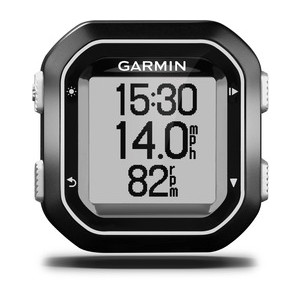
\includegraphics[width=11em]{figuras/cf-lg.jpg}}
    \label{fig:garmin}
\end{figure}
\centerline{Fonte: TEste \textit{Web}}

\section{Trabalhos científicos}
Entre os trabalhos científicos pesquisados estão... \par



% Metodologia
%Arquivo contendo o capítulo Metodologia
\chapter{Metodologia} \label{cap:metodologia}
A primeira etapa para o desenvolvimento da solução...


% Cronograma
%Arquivo contendo o capítulo Cronograma
\chapter{Cronograma} \label{cap:cronograma}
As atividades serão desenvolvidas conforme o cronograma mostrado na Tabela \ref{cronograma}.

%\begin{table}[h]
%\caption{Cronograma de atividades}
%\begin{center}
%\begin{tabular}{l|c|c|c|c}
%\hline
%\multirow{2}{*}{Tarefa} & 
%\multicolumn{4}{c}{2015}\\& Ago & Set & Out & Nov 
%    \\ \hline
%    Levantamento de Requisitos  
%        & x   & ~   & ~   & ~    
%    \\ \hline
%    Prototipação das Interfaces com Usuário
%        & x   & ~   & ~   & ~  
%    \\ \hline
%    Desenvolvimento do \textit{Template} do Sistema
%        & x   & ~   & ~   & ~      
%    \\ \hline
%    Análise do Sistema
%        & x   & ~   & ~   & ~
%    \\ \hline
%    Desenvolvimento do Módulo de Rastreamento de Atividades 
%        & ~   & x   & ~   & ~
%    \\ \hline
%    Desenvolvimento do Lado do Servidor                                 
%        & ~   & x   & ~   & ~
%    \\ \hline
%    Desenvolvimento do Módulo Avatar                        
%        & ~   & x   & ~   & ~
%    \\ \hline
%    Desenvolvimento Módulo Perfil do Usuário
%        & ~   & ~   & x   & ~
%    \\ \hline
%    Desenvolvimento Módulo de Desafios
%        & ~   & ~   & x  & ~
%    \\ \hline
%    Desenvolvimento da Integração com Redes Sociais         
%        & ~   & ~   & x  & ~
%    \\ \hline
%    Finalização dos Testes                                     
%        & ~   & ~   & ~  & x
%    \\ \hline
%    Finalização da Monografia                               
%        & ~   & ~   & ~  & x
%    \\ \hline
%\end{tabular}
%\end{center}
%\label{cronograma}
%\end{table}

% Conclusão
%\input{conclusão.tex}

% carrega o arquivo com as bibliografias e põe o capítulo com as referências neste lugar
\bibliography{bibliografia}

%% a partir daqui, todo capítulo novo é apêndice
%\appendix

%\chapter{Anexos e Apêndices}
%Destinam-se à inclusão de informações complementares ao trabalho, mas que não %são essenciais à sua compreensão. Os Apêndices devem apresentar material %desenvolvido pelo próprio autor, formatado de acordo com as normas. Já os %Anexos destinam-se à inclusão de material como cópias de artigos, manuais, %etc., que não necessariamente precisam estar em conformidade com o modelo, e %que não foram desenvolvidos pelo autor do trabalho.

%importa dicasLatexABNT.tex para o Apêndice 
%\chapter{Dicas de Latex e Normas ABNT}
Esta capítulo apresenta as coisas básicas que precisamos saber para fazer um TCC com Latex utilizando este modelo.

\section{O Básico do Latex}
Novo parágrafo pode ser feito por meio do comando par. \par
Outra forma é deixando uma linha em branco entre dois parágrafos.

Tudo o que está a direita de um \% é um comentário.
% Isto é um comentário
Para inserirmos o símbolo de porcento de forma proposital, precisamos colocar a barra invertida antes: 90\%.

Os caracteres \& \$ \# \% \_ \{ \} \^{} \~{} $\backslash$ são todos especiais e precisam ser escritos como comandos (com uma barra antes).
% tem um web app para ajudar a encontrar outros símbolos neste endereço: http://detexify.kirelabs.org/classify.html

Aspas são digitadas com duas crases no início e duas aspas simples no final: ``Texto entre aspas''

Estilos de fontes: \textbf{negrito}, \textit{itálico}, \textrm{romano}, \textsf{sans serif}, \texttt{maquina de escrever}, \textsc{caixa alta}.

Capítulos, seções e subseções são inseridas com:
\begin{verbatim}
\chapter{Um Capítulo} -> 1. Um Capítulo
\section{Uma Seção} -> 1.1 Uma Seção
\subsection{Uma Subseção} -> 1.1.1 Uma Subseção
\subsubsection{Uma Subsubseção} -> 1.1.1.1 Uma Subsubseção
\chapter*{Um Capítulo} -> Um Capítulo sem numeração
\end{verbatim}
Não se deve utilizar mais do que 4 níveis.

Ambientes são utilizados para definir uma região do texto que haverá tratamento especial:

\begin{verbatim}
O ambiente verbatin significa "ao pé da letra". 
Ex.: & $ # % _ { } ^ ~ $
\end{verbatim}

\begin{center}
O ambiente center escreve centralizado.
\end{center}

\begin{quote}
O ambiente quote é útil para fazer citações.
\end{quote}

Esta é a forma como se descreve itens:
\begin{description}
\item[Item 1] Isto significa uma coisa.
\item[Item 2] Este significa outra coisa.
\end{description}

Esta é a forma como se cita itens:
\begin{itemize}
\item Item 1;
\item Item 2.
\end{itemize}

E esta é a forma como se enumera itens:
\begin{enumerate}
	\item Qual a alternativa correta?
		\begin{enumerate}
			\item esta.
			\item ou esta.
		\end{enumerate}
\end{enumerate}

Fórmulas matemáticas são colocadas dentro de um ambiente matemático. Tudo neste ambiente é considerado elemento numérico e possui uma formatação diferente. Os comandos aceitos também podem mudar.

Equações matemáticas em destaque são inseridas da seguinte maneira:

% tem um web app para ajudar a fazer equações neste endereço: http://mathurl.com/
% ou aqui: http://webdemo.visionobjects.com/#/demo/equation
$$
x=\frac{-b\pm\sqrt{b^2-4ac}}{2a}.
$$

ou 

\begin{equation}
\begin{array}{rcl}
x_2 - x_1 &\geq& b_1 r_1\\
x_2 - x_1 &\geq& b_2 r_2\\
x_2 - x_1 &\geq& b_n r_m\\
b_1 + b_2 + ... + b_n &=& 1
\end{array}
\end{equation}

enquanto equações inline são feitas desta forma: $r_i (1\leq i \leq m)$.

\section{Convenções}
Escreva o título e os capítulos, seções, subseções, etc. sempre com a primeira letra de cada palavra importante em Maiúsculo e o restante em minúsculo. O Latex se encarregará de deixar tudo MAIÚSCULO onde for necessário.

Nenhuma seção deve ficar sem texto.

Utilize siglas para não ter de repetir muitas vezes o mesmo texto. Neste caso, na primeira ocorrência coloque o significado antes e a sigla entre parênteses (aproveitando também para adiciona-la à lista de siglas). Nas demais ocorrências, apenas coloque a sigla. 
Ex.: ...execução do algoritmo de  \textit{Threshold Accepting} (TA) sobre um circuito. A versão do algoritmo de TA utilizada...

Palavras em \textit{English} ou outra lingua estrangeira devem estar em itálico. Utilize \textbf{negrito} quando for necessário destacar alguma coisa.

\section{Figuras e Tabelas}

Todas as figuras e tabelas devem estar referenciadas no texto e com a descrição acima delas. Não são permitidos outros nomes tais como: quadro, imagem, etc.  Comece a descrição com letra maiúscula e faça o restante em minúscula (exceto siglas), terminando com um ponto final.

Se buscada em alguma obra publicada, a citação deve sempre aparecer. Pode ser colocada entre parênteses, como no exemplo da Figura \ref{fig:dsp2}, ou preferencialmente abaixo após a palavra "Fonte: ", como no exemplo da Tabela \ref{tab:comp1}. Observando que na LISTA DE FIGURAS/TABELAS a fonte/citação não deve aparecer.

É possível colocar as figuras de lado e também redimensiona-las através dos parâmetrosdo Latex, como nos exemplos das Figuras \ref{fig:dsp} e \ref{fig:dsp2}. Dê preferência por imagens vetoriais ou em PDF, para não perder qualidade. Procure deixar os textos das figuras com o mesmo tamanho das letras no restante do documento.

\begin{figure} % [h] -> utilize este parâmetro para forçar nesta posição
    \caption{Segundo a ABNT, a descrição deve ficar acima da figura}
    \centerline{\includegraphics[width=20em]{figuras/dsp}}
    \label{fig:dsp}
\end{figure}

\begin{sidewaysfigure}
    % entre colchetes a descrição que vai para a lista de figuras, sem legenda (opcional)
    \caption[Descrição com citação]{Descrição com citação \cite{artigo}}
    \centerline{\includegraphics[width=40em]{figuras/dsp}}
    \label{fig:dsp2}
\end{sidewaysfigure}

As tabelas devem ser ``abertas'' dos lados (sem as linhas laterais), como no exemplo da Tabela \ref{tab:comp1}, isto torna a imagem mais limpa e clara.

% tem um web app para ajudar a fazer tabelas no latex neste endereço: http://truben.no/latex/table/
\begin{table}
    \centering
    \scalefont{0.93} %necessário eventualmente para reduzir o tamanho da tabela
    \caption{Comparação entre X e Y.}
    \begin{tabular}{c|c|c|c|c|c} \hline
        \multirow{2}{*}{\bf{Célula}} & \multirow{2}{*}{\# \bf{Trans.}} & \multicolumn{3}{|c|}{\bf{Largura} ($\mu m$)} & \bf{Tempo Exec. (s)}\\ \cline{3-6} 
         &  & Std. Cell & ASTRAN & \% & ASTRAN \\ \hline \hline
        AND2X4& 6 & 1 & 1,2 & 20 & 10 \\ \hline
        FAD1X4& 28 & 3,6 & 4 & 12 & 750\\ \hline
        FAD1X9& 28 & 4,2 & 4,2 & 0 & 1800\\ \hline
        HAD1X9& 14 & 2,4 & 2,4 & 0 & 30\\ \hline
        HAD1X18& 18 & 2,8 & 2,8 & 0 & 205\\ \hline
        INVX0 & 2 & 0,6 & 0,6 & 0 & 1\\ \hline
        TOTAL& - & 28 & 29 & 3,6 &-\\ \hline
    \end{tabular}
    {\\ Fonte: \cite{artigo}.}
    \label{tab:comp1}
\end{table}

\section{Citações}
Há duas formas de se fazer uma citação: a citação indireta ou livre e a citação direta ou textual. Todas as citações devem trazer a identificação de sua autoria.

No Latex, inserimos citações utilizando o formato bibtex. Para tanto, precisamos catastrar os dados da citação no arquivo .bib e em seguida citarmos no .tex com o comando cite. Colocar preferencialmente em ordem cronológica, com o mais recente por último \cite{livro, artigo, tese, capitulo, paper, site, apresentacao}.

\subsection{Citação Indireta}
Aquela citação na qual expressamos o pensamento de outra pessoa com nossas próprias palavras. Ex.:

Segundo o trabalho de Silva e Santos \citeyearpar{artigo}, o céu é azul porque...

O céu é azul porque... \cite{artigo}.

\subsection{Citação Direta}
São aquelas em que se transcreve exatamente as palavras do autor citado. As citações diretas ou textuais podem ser breves ou longas. São consideradas breves aquelas cuja extensão não ultrapassa três linhas e devem vir entre aspas. As citações com mais de três linhas são chamadas de longas (sem aspas) e devem receber um destaque especial com recuo.  Ex.:

Segundo Fulano, ``Quando a luz passa através de um prisma, seu espectro é dividido em sete cores monocromáticas'' \citeyearpar{artigo}.

\begin{quote}
Quando a luz passa através de um prisma, seu espectro é dividido em sete cores monocromáticas, eis que surge um arco-íris de cores. A atmosfera faz o mesmo papel do prisma, atuando onde os raios solares colidem com as moléculas de ar, água e poeira e são responsáveis pela dispersão do comprimento de onda azul da luz. \cite{artigo}
\end{quote}

Havendo supressão de trechos dentro do texto citado, faz-se a indicação com reticências entre colchetes [...]. De forma similar, para interpelação, acréscimo ou comentário durante a citação, deve-se fazê-lo também entre colchetes. No início ou no fim da citação, as reticências são usadas apenas quando o trecho citado não é uma sentença completa.Ex.:

``Também chamado de corpo do trabalho, [o desenvolvimento] tem por finalidade expor [...] a explicitação do assunto a ser abordado...'' \cite{artigo}.

\section{Notas de Rodapé}
As notas de rodapé\footnote{Nota sobre a palavra rodapé} são usadas nos documentos impressos para explicar ou fazer comentários detalhados.


\end{document}
